\chapter{Related Work}\label{ch:related_work}

In this chapter, we introduce a few other application areas outside of education where the ML2P-VAE method can be applied. Although the development of the method was done with item response theory in mind, there are other fields which have similar goals to IRT where ML2P-VAE can be applied. As this is not the primary focus of this thesis, we introduce the application setting, draw analogues to education and IRT, and analyze some preliminary results.


\section{Health Sciences}
Beck Depression Inventory

-BDI is already connected to IRT
-This is interesting because we can add in other features along with response data.


\section{Sports Analytics}
\sideremark{Consider cutting this section down a lot}
Over the past few decades, sports franchises have become more willing to incorporate technology and analytics into their strategy, both on and off the field. For example, the large availability of data has influenced basketball teams to strive for more efficient offense \sideremark{TODO: citation}. Off the field, a common task is player evaluation. On sports talk shows, TV personalities often argue over who is the ``greatest player of all time''. These arguments are driven by simple in-game measurements as well as more complicated analytics. 

In 2011, the movie ``Moneyball'' brought the topic of sports analytics to the public eye, describing the strategy of the 2002 Oakland Athletics baseball team in finding the best valued players \sideremark{TODO: cite moneyball}. Oakland's approach was to find players who would reasonably increase the team's win total, but were undervalued in terms of salary. In general, the task of player evaluation seeks to quantify the contributions of players.

\subsection{VAE for Player Evaluation}
The ideas of the ML2P-VAE model can be used in this application. Though not all aspects of ML2P-VAE are relevant due to the lack of statistical theory (there is no analogue of IRT models in player evaluation), we can still interpret a hidden layer of the neural network. The goal of this application is to develop new measures for skill quantification of baseball players. This work was originally presented at the Conference on Fuzzy Systems and Data Mining (FSDM) 2019 by Converse et al. \cite{fsdm_paper}.

We use a modified VAE for the task of evaluating baseball players in four offensive skill areas. Baseball was chosen over other sports including football and basketball for various reasons: (a) the availability of data, (b) the popularity of analytics in the sport, (c) the consistency of rules and styles of play over the past \~50 years, and (d) the lack of positional dependency.

The correspondence to IRT is as follows. Instead of responses to items on an exam, simple measurable statistics (hits, walks, etc.) over the course of a season. The latent ability $\theta$ in IRT corresponds with the underlying skills required to produce the measurable statistics. In baseball, the four skills chosen are \textit{contact} (how often does the batter hit the ball), \textit{power} (how hard does the player hit the ball), \textit{baserunning} (is the player good at running the bases), and \textit{pitch intuition} (does the player swing when they are supposed to).

In ML2P-VAE, the core feature which allows for interpretation of the neural network is the $Q$-matrix, relating latent abilities with exam items. A similar binary matrix can be constructed associating underlying baseball skills with measurable statistics. For example, the statistic ``home runs'' requires only the power skill, while avoiding ``strikeouts'' requires both contact and pitch intuition. A full description of the game statistics used can be found in the appendix. \sideremark{TODO: add $Q$-matrix and other stuff to appendix}

This binary matrix determines the non-zero connections between the learned distribution layer (representing baseball skills) and the output layer (reconstructions of the input game statistics). Note that it is reasonable to use a VAE instead of regular autoencoder because it is assumed that among the population of professional baseball players, the distribution of each skill roughly follows a standard normal distribution. This assumption could be altered to allow for correlated underlying skills, but it would be difficult to find an accurate covariance matrix for abstract skills.

\subsection{Experiments}
\sideremark{Should add citation to data}
Data was gathered from Major League Baseball players from 1950-2018, yielding 8,604 samples, where each data point corresponds to a particular player's performance in a particular year. 13 measurable game statistics were chosen as inputs to the VAE: singles (1B), doubles (2B), home runs (HR), runs (R), runs batted in (RBI), walks (BB), intentional walks (IBB), strikeouts (K), sacrifice (SAC), grounded into double play (GDP), stolen bases (SB), caught stealing (CS), and walk/strikeout ratio (BB/K). Each statistic was rescaled using Gaussian normalization so that each input feature was centered at 0 with variance one. Additionally, the game statistics strikeouts and caught stealing were multiplied by $-1$ for each observation so that a larger number is more desirable. As in the ML2P-VAE architecture, the decoder weights are constrained to be non-negative, so that a higher skill value can only increase the reconstructed in-game statistics.

Since this is an unsupervised method with the goal of creating \textit{new} skill measures, it is difficult to evaluate the obtained results. Instead, we take the more commonly used baseball statistics contact rate (CR), speed score (SPD), isolated power (ISO), and on-base percentage (OBP) to compare with the skills \textit{contact}, \textit{baserunning}, \textit{power}, and \textit{pitch intuition}, respectively. More informationon how these measures are calculated can be found in the appendix. \sideremark{TODO: add to appendix}

\begin{figure*}[h!]
\centering
\minipage{0.5\textwidth}
    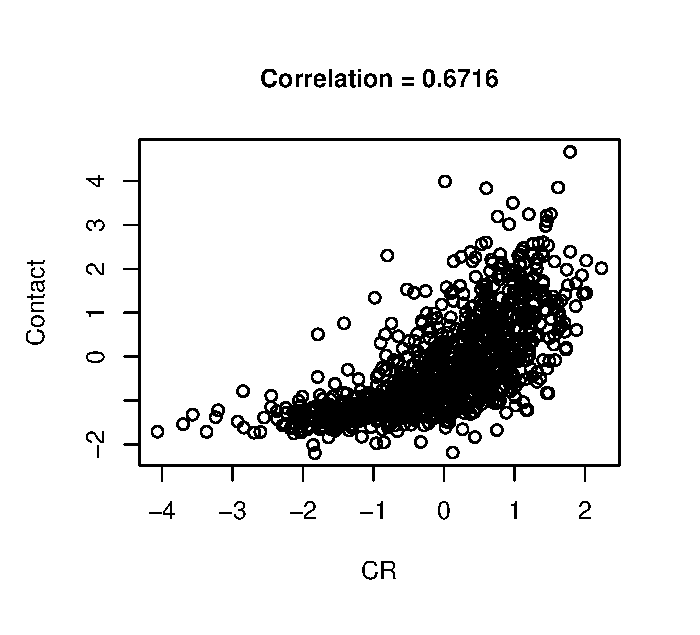
\includegraphics[width=.85\textwidth]{img/fsdm_results/contact_corr.eps}
\endminipage\hfill
\minipage{0.5\textwidth}
    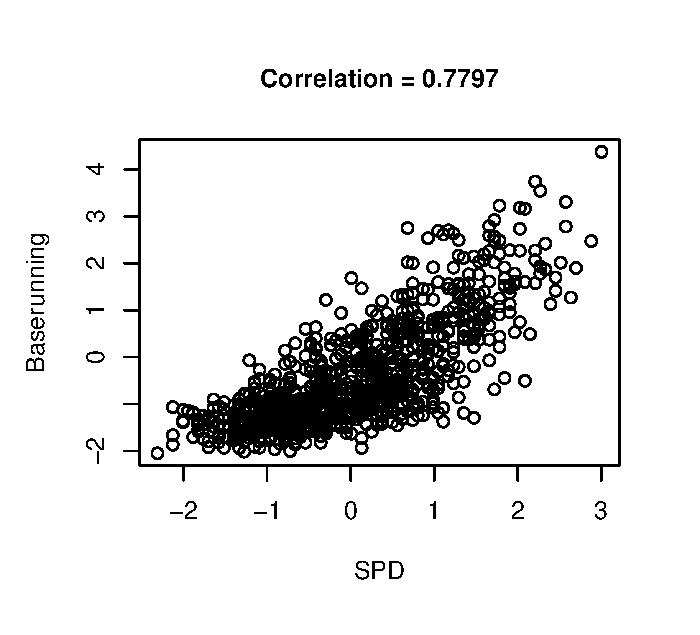
\includegraphics[width=.85\textwidth]{img/fsdm_results/baserun_corr.eps}
\endminipage
\hfill
\minipage{0.5\textwidth}
    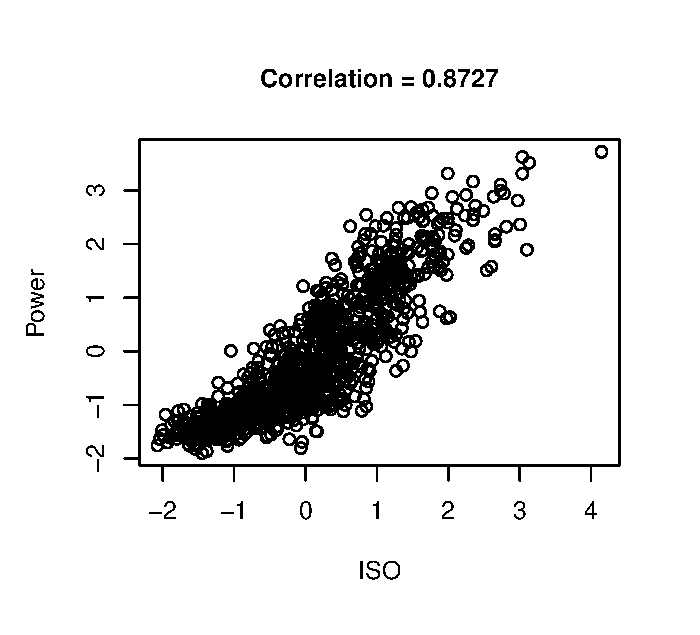
\includegraphics[width=.85\textwidth]{img/fsdm_results/power_corr.eps}
\endminipage\hfill
\minipage{0.5\textwidth}
    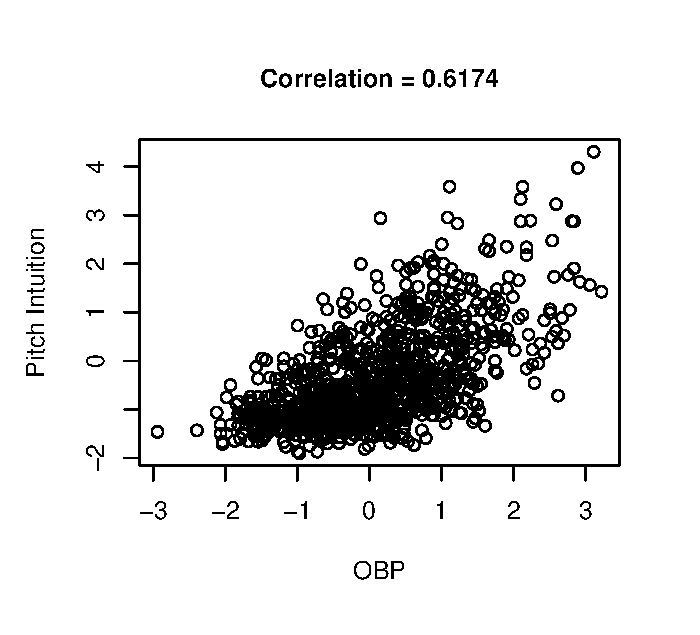
\includegraphics[width=.85\textwidth]{img/fsdm_results/pitch_intuit_corr.eps}
\endminipage\hfill
\caption{Each latent skill's estimates plotted against its evaluation statistic.}
\label{fig:baseball}
\end{figure*}

Each skill is plotted against its evaluation statistic in Figure \ref{fig:baseball} \cite{fsdm_paper}. Note that each of the four plots display high correlation, but do not match exactly. This is desirable in the sense that our new skill quantifications do in fact measure what they are intended to measure, but give new insights and ranking for each player. Though these results could be improved, it is clear that variations of the ML2P-VAE model can be applied in areas other than education.


